%************************************************
\chapter{Introduction to nucleic acid structure }\label{ch:introduction}
%************************************************
\section{Survey}
In Biology, organisms are the living entities that consist of organs and the organs are made of tissues. The fundamental building blocks of the organisms that form tissues are cells. Cells consist of various molecules and molecular biology is the field of science that studies cells at the molecular level. 

Molecules in the cell participate in various biochemical reactions to maintain the proper structure and function of the cell. There are micromolecules that are small molecules of low weights, they often refer to monomers. Many micromolecules can join together to form more complex molecules called macromolecules. There are four essential macromolecules in the cell---the nucleic acids that carry the genetics blueprint and the instructions for the functioning of the cell---the lipids that---the proteins that are one of the most abundant organic molecules in the living systems. They contribute in many functional activities: enzymatic catalyses, contractility, formation of selectively permeable membranes, reversible binding and transport, and immunological activities.---the carbohydrates that are essential part of our diet. They provide energy to the body; grains, fruits and vegetable are all considered to be natural source of carbohydrates.
 
Our work focuses on the nucleic acids. The nucleic acids are made up of small repetitive micromolecules called nucleotides. Genetic information necessary to specify the proteins needed by the organisms is contained in a nucleic acid call deoxyribonucleic acid (DNA) or, in some cases for some viruses in the ribonucleic acid (RNA). 
%\section{Macromolecules: From DNA to RNA}

\section{Deoxy-nucleic Acids (DNAs)}

DNAs are macromolecules contained in the nucleus of eukaryotic cells that allow storing information with the help of nucleotides.  Nucleotides consist of a five carbon sugar, a phosphate group, and a nucleobase. There are four nucleotides in the DNA, each of them distinguished by the nucleobase they have: A for Adenine , T for Thymine, G for Guanine, and C for Cytosine. Even though the basis blocks constituting the DNA was known for many years, it was only in 1953 that James Watson and Franklin Crick succeeded in putting them together and suggested a reasonable DNA structure. Their work relayed on DNA X-ray diffraction pattern produced by Rosalind Franklin and Maurice Wilking and the data from Erwin Charganp. Their work revealed for the first time that the structure of DNA molecules has helical chains, each coiled round the same axis where the chain consists of phosphate dieter groups. The two chains are held together by the purimide and pyrimidine bases, they are joined together in pairs, a singlle base from the other chain bonded to a single base from the other chain. For the bonding to occur one of the pair must be Ademine and thymine or Guanine and Cytosine. The complementary pairing of the bases was then compatible with Chargaff's empirical rules---the amount of pyrimidine nucleotides (T+C) always equals the total number of purine nucleotides (A+G). 
\graffito{\includegraphics[width=1\linewidth]{../res/images/dna.png}
		Helical representation of DNA structures.}

The elucidation of DNA structure by Watson and Crick has then motivated many other scientists for futher investigations and gave rise to a modern molecular biology. Later in the same year, Watson and Crick formulated the central dogma of molecular biology that describes the flow of information between DNA, RNA, and proteins.  Fig 2 illustrates the dogma in two steps: from DNA to mRNA through transcription, from mRNAs to proteins through translation. Since this central dogma was proposed, more works have been done in investigating  in details each steps of the Fig 2. DNAs are transcribed into RNA molecules (messenger RNAs) that contain the same information as the template DNAs, and subsequently these RNA messengers are translated into proteins according to the genetic code [Miller et al., 2009]. 

\section{non-coding RNAs and their biological implications} 
So far in this work, RNAs have been considered as paying the same common role as DNAs which is the genetic information memory. But not all RNAs are translated into proteins, in other terms not all RNAs are mRNAs. There are mainly two RNA's groups: coding RNAs (cRNAs) that are translated into proteins and non-coding RNAs that are not translated into proteins.  In the previous section, we introduced the central dogma of microbilogy which describe the flow of informations in the living systems. In other terms information flows from nucleic acids to proteins and not vice versa. It therefore, appears that DNAs and proteins are vital components of living systems.  But during the transcription and the translation steps in the information flow, there are some functions performed by non-coding RNAs such as ribosomal RNA (rRNAs) and transfer RNAs (tRNAs). The study of such RNAs revealed that rRNAs rather than ribosomal proteins catalyse the synthesis of proteins  (i.e.  the polymerization of amino acids), distinguish between correct and incorrect codon-anticodon pairs and prevent the premature hydrolysis of peptidyl-tRNAs. [Ref Moore PB, Steiz TA. The role of RNA in the synthesis of proteins. In: Gesteland RF, Cech TR, Atkins JF, editors. The RNA world. 3rd edition. Cold Spring Harbor (NY, USA): Cold Spring Harbor Laboratory Press; 2005. p. 257–85.]. Such studies suggest that RNAs are the actual catalysts of protein synthesis even though proteins remain the common catalysts of various chemical reactions occurring in the cell. This implies also that not only proteins, but also RNAs can function as efficient catalysts.  In addition to protein synthesis, experiments in vitro evolution have shown that RNA molecules can catalyse a variety of chemical reactions relevant to biological processes such as RNA replication, nucleotide synthesis, thymidylate synthesis, lipid synthesis, and sugar metabolism (see Robertson DL, Joyce GF. Selection in vitro of an RNA enzyme that specifically cleaves single-stranded DNA. Nature , Ellington AD, Chen X, Robertson M, Syrett A. Evolutionary origins and directed evolution of RNA. The International Journal of Biochem-
istry \& Cell Biology ). Therefore, RNA molecules can perform functions partially equivalent to those performed by proteins. 
\graffito{
		\scalebox{0.95}{
			
			\chemname[1cm]{\chemfig{
					-[,1.202,,,line width=3.5pt, shorten <=-.05pt, shorten >=-.05pt](-[:-90,,,,line width=1.5pt, shorten >=.5pt]OH)% 2
					>[:44.6,0.521](-[:90, 3.3]{\textcolor{blue}{Nucleobase}})
					-[:167]\chembelow[35pt]{O}{Ribose}
					-[:193,0.998]
					(
					-[:90](-[,0.1,,,draw=none]\chemabove[1ex]{}{\textcolor{gray}{5'}})
					-[::90,1.,,,red](-[::0,,,,red]\color{red}{P}(-[2,,,,red]\color{red}{O^{-}})(-[4,1.3,,,red]\color{red}{O^{-}})(=[6,,,,red]\chembelow{\color{red}{O}}{\textcolor{red}{Phosphate}}))
					)
					(
					<[:315.6,0.522](-[:-90,,,,line width=1.5pt, shorten >=.5pt]OH)(-[::-150,0.4,,,draw=none]\chembelow[1ex]{}{\textcolor{gray}{3'}})
					)
			}	}{Structure of an RNA nucleotide}
		}
	}

Several works revealed also that DNAs can perform some catalytic reactions, but the implication of RNAs in most of the vital chemical reactions in living systems and its broader range of chemical reactions have motivated many scientists in the last decay to study RNA molecules in more details as an independent entity.  This section of our work focuses on the biochemistry of RNA structure in general, and especially on highlighting the biological importance of non-coding RNAs. 
\subsection{Biochemistry of RNA molecules}\label{sec:rna_biochemical}

RNAs are synthesized from DNAs through a process often termed the transcription. The transcription process takes place in cell's nucleus and it is performed by RNA polymerases. Depending on the type of cells, there are many (or one) types of RNA polymerase responsible for the synthesis of a specific type of RNAs. During transcription, an RNA polymerase uses the 3’-5’ DNA template strand to synthesize a 5’-3’ RNA strand with complementary nucleotides. Similar to DNAs, nucleotides constitute the basis of  RNA molecules and each nucleotide consists of a phosphate residue, a pentose sugar and a nucleobase. We also find four different nucleotides in RNA, each of them distinguished by the nucleobase they have: Adenine (A), Cytosine (C), Guanine (G) and Uracil (U) which replaces Thymine in DNA. Figure \ref{fig:nucleotide} depicts the chemical structure of each of the four different nucleobases found in RNA. Chemically, a nucleotide is a nucleoside, which has a (mono, di, trip) phosphate residue bound to its 5'-carbon atom. The common chemical structure of a nucleotide is depicted on the right side of the page. By convention, the carbon atoms of the pentose sugar in nucleotides are numbered with primes.

\begin{figure}
	\begin{minipage}[tb!]{.5\linewidth}
		\centering 
		\scalebox{0.9}{
			\chemfig{
				-[,1.202,,,line width=3.5pt](-[:-90,,,,line width=1.5pt]OH)% 2
				>[:44.6,0.521](-[:90] \color{blue}{N}*5(-[,,,,blue]*6(-[,,,,blue]\color{blue}{N}=[,,,,blue]-[,,,,blue]\color{blue}{N}=[,,,,blue](-[:90,,,,blue]\color{blue}{NH_2})-[,,,,blue]-[,,,,blue])=[,,,,blue]-[,,,,blue]\color{blue}{N}=[,,,,blue]-[,,,,blue]))
				-[:167]O
				-[:193,0.998]
				(
				-[:90](-[,0.1,,,draw=none]\chemabove[1ex]{}{\textcolor{gray}{5'}})
				-[::90]O(-[::0]P(-[2]O^{-})(-[4]O^{-})(=[6]O))
				)
				(
				<[:315.6,0.522](-[:-90,,,,line width=0.5pt]OH)(-[::-150,0.4,,,draw=none]\chembelow[1ex]{}{\textcolor{gray}{3'}})
				)
			}	
		}
		\subcaption{Adenosine 5'􏱈-monophosphate}\label{fig:adenine}
	\end{minipage}%
	\begin{minipage}[b]{.5\linewidth}
		\centering
		\scalebox{0.9}{\chemfig{
				-[,1.202,,,line width=3.5pt, shorten <=-.05pt, shorten >=-.05pt](-[:-90,,,,line width=1.5pt, shorten >=.5pt]OH)% 2
				>[:44.6,0.521](-[:90] \color{blue}{N}*6(-[,,,,blue](=[,,,,blue]\color{blue}{O})-[,,,,blue]\color{blue}{NH}-[,,,,blue](=[,,,,blue]\color{blue}{O})-[,,,,blue]=[,,,,blue]-[,,,,blue]))
				-[:167]O
				-[:193,0.998]
				(
				-[:90](-[,0.1,,,draw=none]\chemabove[1ex]{}{\textcolor{gray}{5'}})
				-[::90]O(-[::0]P(-[2]O^{-})(-[4]O^{-})(=[6]O))
				)
				(
				<[:315.6,0.522](-[:-90,,,,line width=1.5pt, shorten >=.5pt]OH)(-[::-150,0.4,,,draw=none]\chembelow[1ex]{}{\textcolor{gray}{3'}})
				)
		}}
		\subcaption{Uridine 5'􏱈-monophosphate}\label{fig:uracil}
	\end{minipage}
	\begin{minipage}[b]{.5\linewidth}
		\centering
		\scalebox{0.9}{	\chemfig{
				-[,1.202,,,line width=3.5pt, shorten <=-.05pt, shorten >=-.05pt](-[:-90,,,,line width=1.5pt, shorten >=.5pt]OH)% 2
				>[:44.6,0.521](-[:90]\color{blue}{N}*6(-[,,,,blue](=[,,,,blue]\color{blue}{O})-[,,,,blue]\color{blue}{N}=[,,,,blue](-[,,,,blue]\color{blue}{NH_2})-[,,,,blue]=[,,,,blue]-[,,,,blue]))
				-[:167]O
				-[:193,0.998]
				(
				-[:90](-[,0.1,,,draw=none]\chemabove[1ex]{}{\textcolor{gray}{5'}})
				-[::90]O(-[::0]P(-[2]O^{-})(-[4]O^{-})(=[6]O))
				)
				(
				<[:315.6,0.522](-[:-90,,,,line width=1.5pt, shorten >=.5pt]OH)(-[::-150,0.4,,,draw=none]\chembelow[1ex]{}{\textcolor{gray}{3'}})
				)
			}
		}
		
		\subcaption{Cytidine 5'􏱈-monophosphate}\label{fig:cytosine}
	\end{minipage}%
	\begin{minipage}[b]{.5\linewidth}
		\centering 
		\scalebox{0.9}{	
			\chemfig{
				-[,1.202,,,line width=3.5pt, shorten <=-.05pt, shorten >=-.05pt](-[:-90,,,,line width=1.5pt, shorten >=.5pt]OH)% 2
				>[:44.6,0.521](-[:90] \color{blue}{N}*5(-[,,,,blue]*6(-[,,,,blue]\color{blue}{N}=[,,,,blue](-[,,,,blue]\color{blue}{NH_2})-[,,,,blue]\color{blue}{NH}=[,,,,blue](=[:90,,,,blue]\color{blue}{O})-[,,,,blue]-[,,,,blue])=[,,,,blue]-[,,,,blue]\color{blue}{N}=[,,,,blue]-[,,,,blue]))
				-[:167]O
				-[:193,0.998]
				(
				-[:90](-[,0.1,,,draw=none]\chemabove[1ex]{}{\textcolor{gray}{5'}})
				-[::90]O(-[::0]P(-[2]O^{-})(-[4]O^{-})(=[6]O))
				)
				(
				<[:315.6,0.522](-[:-90,,,,line width=1.5pt, shorten >=.5pt]OH)(-[::-150,0.4,,,draw=none]\chembelow[1ex]{}{\textcolor{gray}{3'}})
				)
			}
		}
		
		\subcaption{Guanosine 5'􏱈-monophosphate}\label{fig:guanine}
	\end{minipage}%
	
	
	\caption{RNA nucleotides. Adenine and guanine belongs into the chemical class of purine molecules and the uracil and thymine in the class of pyrimidines}\label{fig:nucleotide}
\end{figure}
RNA molecules are simply represented as list of nucleobase characters and their functions often depend on their complex multidimensional structures. The different nucleotides composing the RNA molecule are attached by 5'-3' phosphatediester bonds between ribose to form the primary structure of RNA. The direction of the chain is conventionally designed as 5' to 3' e.i. from 5'-phosphate of the first sugar of the backbone to the 3'-hydroxyl of the last sugar in the sequence.  The process in which RNA sequences are mapped to their corresponding structures is called RNA folding. In nature, RNA folding is thought to be hierarchical [2,20 from lemerlaeu GECCO]. Nucleotides form a chain given their sequence of bases (primary structure), RNAs fold into secondary structures, such as stem loops and helices, before folding into higher level (tertiary and quaternary) structures. Our work is restricted here to the secondary level of RNA structures. In contrast to the RNA primary structure, the secondary structure consists of a list of nucleobase pairs and the base pairs are formed via hydrogen bonds between the bases.  Different interactions are possible between the bases depending on the structure level considered: At the secondary level, we have the Watson-Crick (or canonical) pairs \cite{seeman1976rna, rosenberg1976rna} (A-U and G-C), the Wobble (or  non-canonical) (G-U) pairs that occur with reduced frequency. Figure \ref{fig:basepairing} shows the chemical base pairs for the Watson-Crick and Wobble interaction. 


\begin{figure}
	\begin{minipage}[b]{1.0 \linewidth}
		\centering
		\chemfig{
			R-[::42] N*5(
			%(-H)
			-(*6(
			-N=-N?[h1]
			=(-N([::60]-H)([::-60]-H?[h0]))-=
			))
			--N=-
			)
			*5(-[,,,,draw=none](*6(-[,,,,draw=none]-[,,,,draw=none]-[,,,,draw=none](-[,,,,draw=none]))))
			\phantom{A}-[,1.95,,,draw=none]
			-[::-60,2,,,draw=none]-[,2,,,draw=none]-[::120,,,,draw=none]
			N*6(%(-H)
			-=-(=O?[h0,,{dash pattern=on 1pt off 4pt}, {line width=1.5pt}, gray])-N(-H?[h1,,{dash pattern=on 1pt off 4pt}, {line width=1.5pt}, gray])-(=O?[h2,,{dash pattern=on 1pt off 4pt}, {line width=1.5pt}, gray])-)
			-[::180]R
		}
		\subcaption{Adenine-Uracil Interaction}
	\end{minipage}%
	
	\begin{minipage}[b]{1.0 \linewidth}
		\centering
		\chemfig{
			R-[::42]	N*5(
			%(-H)
			-(*6(
			-N=(-{NH_2})
			-N(-H?[h2])
			-(=O?[h1])-=
			))
			--N=-
			)
			*5(-[,,,,draw=none](*6(-[,,,,draw=none]-[,,,,draw=none]-[,,,,draw=none](-[,,,,draw=none]))))
			\phantom{A}-[,1.95,,,draw=none]
			-[::-60,2,,,draw=none]-[,2,,,draw=none]-[::120,,,,draw=none]
			*6()
			N*6(%(-H)
			-=-(-N([::60]-H?[h1,,{dash pattern=on 1pt off 4pt}, {line width=1.5pt}, gray])([::-60]-H))=N?[h2,,{dash pattern=on 1pt off 4pt}, {line width=1.5pt}, gray]-(=O?[h3,,{dash pattern=on 1pt off 4pt}, {line width=1.5pt}, gray])-)
			-[::180]R
		}
		\subcaption{Guanine-Cytosine Interaction}
	\end{minipage}%
	
	\begin{minipage}[b]{1.0 \linewidth}
		\centering
		\chemfig{
			R-[::42]	N*5(
			%(-H)
			-(*6(
			-N=(-{NH_2})
			-N(-H?[h2])
			-(=O?[h1])-=
			))
			--N=-
			)
			*5(-[,,,,draw=none](*6(-[,,,,draw=none]-[,,,,draw=none]-[,,,,draw=none]-[,,,,draw=none](-[,,,,draw=none]))))
			\phantom{A}-[,2.95,,,draw=none]
			-[::-60,2,,,draw=none]-[,2,,,draw=none]-[::120,,,,draw=none]
			N*6(%(-H)
			-=-(=O?[h0,,{dash pattern=on 1pt off 4pt}, {line width=1.5pt}, gray])-N(-H?[h1,,{dash pattern=on 1pt off 4pt}, {line width=1.5pt}, gray])-(=O?[h2,,{dash pattern=on 1pt off 4pt}, {line width=1.5pt}, gray])-)
			-[::180]R
		}
		\subcaption{Guanine-Uracil Interaction}
	\end{minipage}
	
	\caption{RNA base pair interactions.}\label{fig:basepairing}
\end{figure}
Additionally to the canonical and non-canonical pairs, we also find crossing or pseudoknotted interactions in natural RNA and they play vital roles in realising biological functions. Pseudoknots occur when two canonical or non-canonical interactions cross each other \cite{beyongWCpairs}.  Even though pseudoknots are often considered to be the beginning of the interaction between the secondary and tertiary levels of RNA structures, we consider them to be part of the secondary structure. Therefore, two main secondary structure definitions are considered in this work: a pseudoknot-free one in which only canonical interactions with no crossing pairs are allowed and a second one where canonical interactions with possible crossing pairs are allowed. 

\begin{figure}
	\includegraphics[width=1.0 \linewidth]{../res/images/arnaque/pk_type}
	\caption{RNA pseudonotted interactions}
\end{figure}

\subsection{Biological function of non-coding RNAs}\label{sec:custom}

This section may be included in the section 1.1.  Nevertheless, this will provide a particular introduction to some non-coding RNAs and underlay their biological significances. e.g. Aptamers \& Riboswitches, SELEX, etc...

\section{Bioinformatic definitions and RNA concepts.}
In order to computationally study and analyse RNA molecules, a more formal representation of RNAs and bioinformatic definitions are required. We provide in this section, formal definitions and concepts that will support the result presented in this thesis.

\paragraph{\textbf{Definition 1}} ( RNA sequence): Let $S$ be an RNA sequence of length $L$.  More formally, $S$ consists of an ordered sequence of nucleotides that can be represented as:~ \[S\ =\ \left(S_1,...,S_L\right)\ where\ S_i\in\left\{A,C,G,U\right\}\]~
\(S\)~is often known as the primary structure of RNA.

\paragraph{\textbf{Definition 2} } (RNA pseudoknot-free secondary structure): Given an RNA sequence $S\in \{A,C,G,U\}^L$, let $P=\big \{(i,j) \colon i<j \big \}$ be the list of possible pairing positions over the sequence $S$. A pseudoknot-free secondary structure $P_{\sigma} \subset P $ of such sequence $S$ is a list of base pairs  with the following constraints:

\begin{enumerate}
	\item A nucleotide (sequence position) can only belong to a single pair, i.e. $\forall (i,j), (k,l) \in P_{\sigma}$ with $i<k \colon i=k \Rightarrow j=l$.
	\item Paired bases must be separated by at least three
	bases. i.e. \(\forall (i,j) \in \sigma \Rightarrow \) \(j-i>3\).
	\item There are no pseudoknots, i.e. $ \nexists \left(i,j\right), \left(k,l\right) \in P_{\sigma} $
	~with~\(i<k<j<l\),
	\item The base pairs consist almost exclusively of Watson–Crick ($C–G$ and $A–U$) pairs and Wobble ($G–U$) pairs. i.e. $\forall \left(i,j\right) \in P_{\sigma} \Rightarrow S_iS_j \in \left\{GC,CG,AU,UA,GU,UG\right\}$,

\end{enumerate}
\paragraph{\textbf{Definition 3} } (Secondary structure representation): A graphical way of representing an RNA secondary structure. Let $P_{\sigma}$ be a secondary structure of an RNA sequence $S$ of length $L$. There are several representations of $P_{\sigma}$. 
\begin{itemize}
	\item Dot-bracket (Or string) representation: In a this representation, the secondary structure $P_{\sigma}$  is complactly stored in a string $\sigma$ consisting of dots and matching brackets. i.e.  $\sigma$ is a string of length $L$ over the alphabet $\Delta_{\sigma}= \big\{ (,),[,],\{,\},<,>,.\big\}$ where, at each unpaired positions we have a dot '.' at the corresponding string position, and $\forall (i,j) \in P_{\sigma}$ we have an opening bracket at position $\sigma_i$ and a closing bracket at position $\sigma_j$. We denote $\sigma}$ the string representation of the structure $P_{\sigma}$.
	\item Planar representation: it is the common way of representing an RNA secondary structure in which $\sigma$ is presented as a graph with each vertex representing a nucleotide  and an edge connecting consecutive nucleotides and base pairs. 
	\item Circular (or circle ) representation: similar to planar representation, $P_{\sigma}$  is represented as a graph but drawn in the plane in such a way that all vertices are arranged on a circle and the edges representing base pairs lie inside the circle. In a pseudoknot-free secondary structure circular representation, the edges do not intersect. 
	\item Linear representation: In this representation, $P_{\sigma}$  is a graph in which the nucleotides are arrange consecutively in a line and the edges representing base pairs form semi-circle  that do not intersect for pseudoknot-free structure.
	\item Mountain representation:  it is mostly used for representing large structures.$P_{\sigma}$  is presented in a two-dimensional graph, in which the $x$-coordinate is the position $k$ of the nucleotide in the sequence $S$ and the $y$-coordinate the number $m(k)$ of base pairs that enclose nucleotide $k$.
	\item Tree representation: $P_{\sigma}$  is drawn as a tree in which internal nodes are the base pairing positions and the leaves are the unpaired positions. The dot-bracket representation is also often considered as a tree represented by a string of parenthesis (base pairs) and dots for the leaf nodes (unpaired nucleotides). 
	\item Shapiro representation: it allows representing the different elements composing $P_{\sigma}$  by single matching brackets and the components are labelled with H(Hairpin), B(Bulge), I (interior loop),M (multi-loop) and S (stacking loop).
\end{itemize}
Figure \ref{fig:representation} shows some examples of RNA secondary structure representation.
\begin{figure}
	\includegraphics[width=1.0 \linewidth]{../res/images/arnaque/intro/RNA_reps}
	\caption{RNA secondary structure representation}\label{fig:representation}
\end{figure}

\paragraph{\textbf{Definition 4} }(Secondary structure loop):  Given a secondary structure $\sigma$ over an RNA sequence $S$ of length $L$, there exists a unique decomposition of $\sigma$ into a set of loops $\mathcal{L}_{\sigma}$, where loops are the faces of its planar drawing. Each loop is characterised by its length $\mathcal{l}$ (the number of unpaired nucleotides in the loop) and its degree $k$ (the number of base pairs delimiting the loop, including the closing loop pair). 
%For the seek of formality, let us consider $\mathcal{P}_{\sigma} =  \mathcal{P}_{bp} \cup \mathcal{P}_{b}$, where $\mathcal{P}_{b} = \big{\{} i | \sigma_i = '.'\big{\}}$ and $\mathcal{P}_{bp} = \big{\{} i | \sigma_i \in \{(', ')' \}'\big{\}}$. We denote $\phi_{i,j}$ a loop of a secondary structure $\sigma$. 
Therefore, $\forall \phi \in \mathcal{L}_{\sigma} \Rightarrow \phi = \phi_p \cup \phi_u$ where $\phi_p$ and $\phi_u$ denote respectively the set of loop base pairs and the unpaired positions. $\phi_p$ contains the closing loop and the interior loop pairs. We say $(i,j) \in \phi_p$ is a closing pair if and only if $\forall \phi_p \ni (i',j') \neq (i,j) \colon i<i'<j'<j$.
\begin{enumerate}
	\item Interior loop: a loop with degree $k=2$ i.e $|\phi_p|=2$ and $\phi_u \in \{P_{\sigma} \cup \emptyset\}$.
	\item Stacking pair: an interior loop of length $l=0$ i.e. $\phi_p=\{(i_1,j_1), (i_2, j_2)\}$ where, $(i_1, j_1)$ is a closing pair  and $(i_2, j_2)$ is an interior pair and,  $\phi_u=\emptyset$.
	\item Hairpin Loop: Any loop of degree $k=1$.  i.e $\phi_p=\{(i_1,j_1)\}=\phi_c$ and  $\phi_o \neq \emptyset$.
	\item Bulge loop: a special case of interior loop in which there are unpaired bases only on one side. i.e  $\phi_p=\{(i,j), (l, k)\}$ with $i \neq k, j\neq l$ one of the following assumption holds: 
		\begin{itemize}
			\item If $\exists i'\in \phi_u | i<i'<j \Rightarrow \nexists k'\in \phi_u | k<k'<l$ 
			\item If $\exists k'\in \phi_u | k<k'<l \Rightarrow \nexists i'\in \phi_u | i<i'<j$ 
		\end{itemize}
	\item Multi-loop: Any loop with degree $k>2$ i.e.  $\phi_p=\{(i_1,j_1), (i_2, j_2), \dots, (i_k, j_k)\}$  and $\phi_u \in \{P_{\sigma} \cup \emptyset\}$.
	\item Exterior loop: a loop in which all the positions are not interior of any pair i.e. $\phi_c=\emptyset$ and $\phi_o \neq \emptyset$.
\end{enumerate}

\begin{figure}[H]
	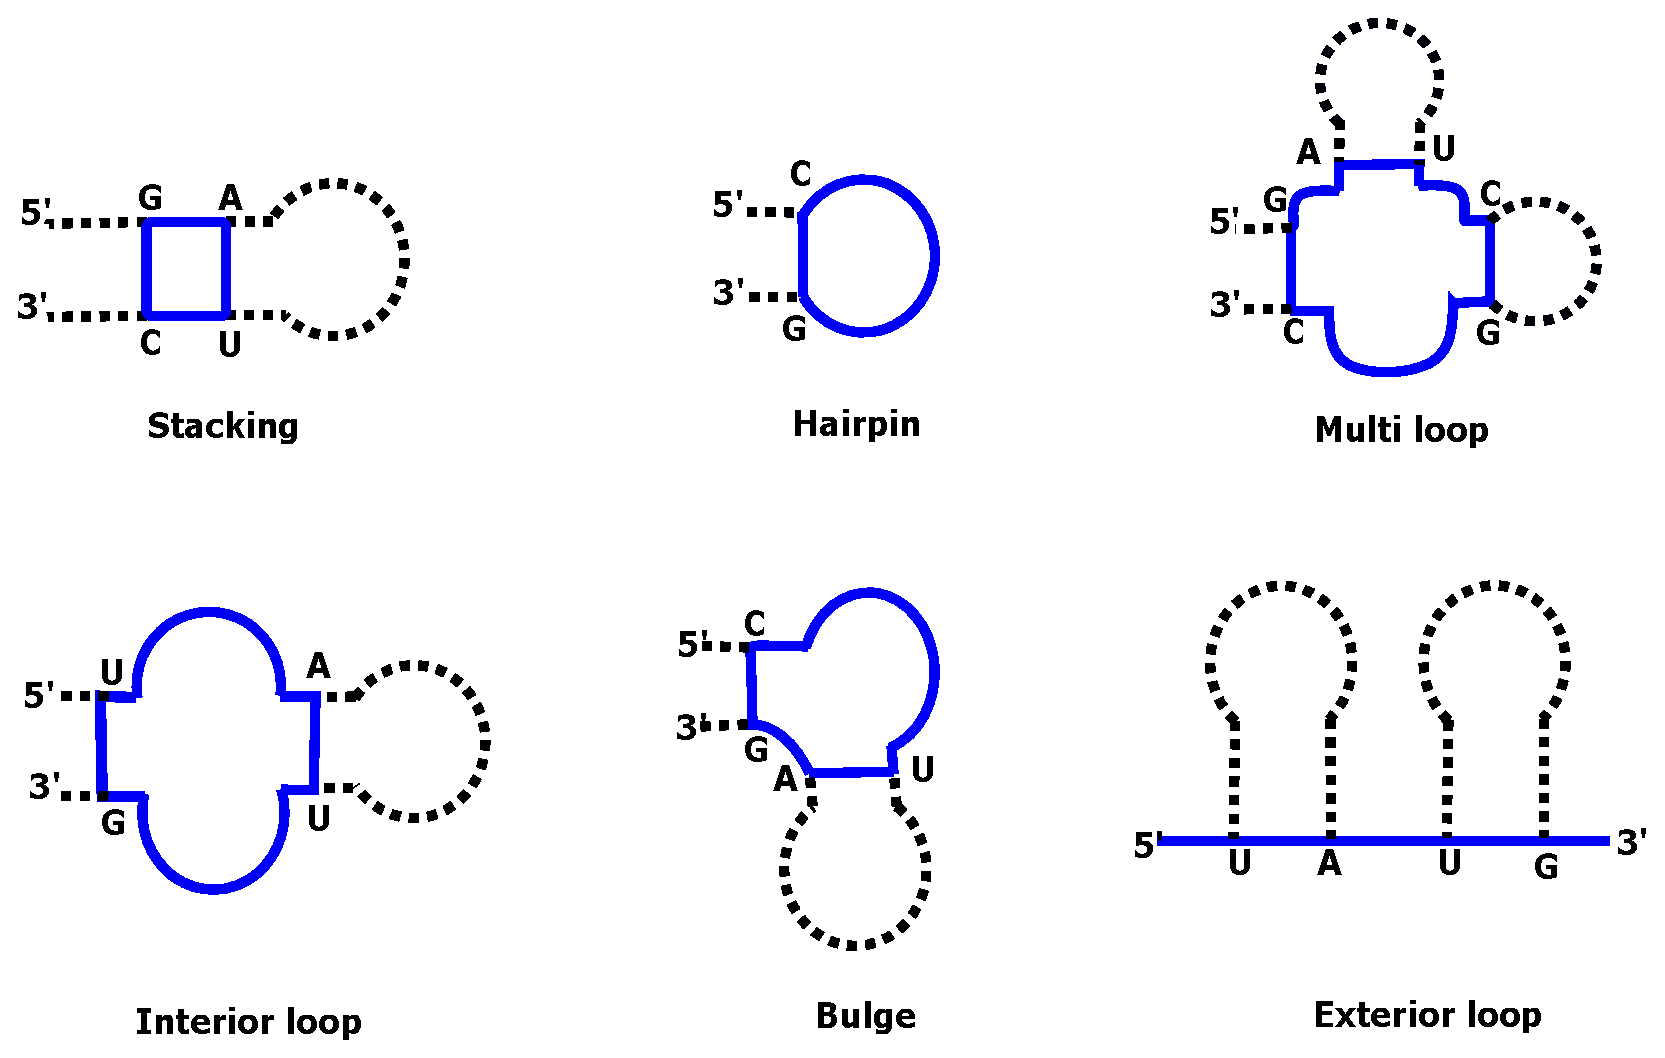
\includegraphics[width=1.0 \linewidth]{../res/images/arnaque/intro/loops}
	\caption{RNA secondary structure loop decomposition}\label{fig:loops}
\end{figure}

\paragraph{\textbf{Definition 5}} (Free Energy of an RNA secondary structure):  it defines the thermodynamic stability of the secondary structure $\sigma$ and it is denoted \(\Delta G_{\sigma}\). \(\Delta G_{\sigma}\) is the free energy difference with respect to the completely unfolded state. The free energy of a secondary structure is computed using the According to the additivity principle \cite{dill97_addit_princ_bioch}, the free energy of a structure can be approximated by the sum of its constituent loops free energies. Many models allow to compute the free energies of those constituent loops, but the dominant one is the nearest-neighbor loop energy model \cite{turner09_nndb}. This model associates tabulated free energy values to loop types and nucleotide compositions; the Turner2004 \cite{mathews2004incorporating} is one of the most widely used parameter sets. This structure decomposition allows an efficient dynamic programming algorithm that can determine the minimum free energy (MFE) structure of a sequence in the entire structure space. The gold standard for free-energy-based predictions is usually the MFE; however, it represents one structural estimate among many others, such as the maximum expected accuracy (MEA).    

\textbf{Definition 4} (Structure Ensemble):

\textbf{Definition 3} (MFE secondary structure): To predict biologically relevant structures, most computational methods search for structures that minimize this free energy.

\textbf{Definition 5} (Secondary structure probability)



\textbf{Definition 6} (Base pair probability): 

\textbf{Definition 7} (Partition function of RNA) : 

\textbf{Definition 8} (Base pair probability matrix): 

\textbf{Definition 9} (Neutral set of RNA sequences) : 

\textbf{Definition 10} (Neutral Network): 

\textbf{Definition 11}  (PPV) : 

\textbf{Definition 12} (FPV) : 

\textbf{Definition 13 } (FFT) : 

\textbf{Definition 14} (Hamming Distance between two SS): 

\textbf{Definition 15} Ensemble defect (ED) \citep{zadeh2011nucleic}: Here, we use the ED as a second objective function for refinement after having at least one sequence that folds into the target in the current population. It is defined as follows: ~

\begin{equation}
\label{ed}
\begin{split}
ED(\phi, \sigma*) &= \sum_{\sigma \in \Gamma}{p(\phi, \sigma)d(\sigma, \sigma*)}\\
&= L - \sum_{1<i,j<L} P_{i,j}(\phi)S_{i,j}(\sigma*)
\end{split}
\end{equation}

where~\(P_{i,j}\)~is the base pair probability matrix and~\(S(s)\)~is the structure matrix with entries~\(S_{i,j} \in  \{ 0, 1\}\). If the structure~\(s\)contains pair~\(\{i ,j\}\), then~\(S_{i,j}(s) = 1\)~otherwise \(S_{i,j}(s) = 0\).

\textbf{Definition 16} Normalized Energy Distance (NED): the difference between
the energy of a given sequence~\(\phi\)~evaluated to fold
into a target structure~\(\sigma*\)~and the minimum free energy
of the sequence in its structural ensemble~\(\Gamma\).~ The value is normalized over all the sequences in a given population $P$.  


\begin{equation}
\label{ned}
NED(\phi, \sigma*) = [1-\Delta E_{norm}(\phi, \sigma*)]^p \text{   } \forall p>1
\end{equation}
where,
\begin{equation}
\Delta E_{norm}(\phi, \sigma*) = \frac{\Delta E(\phi, \sigma*) }{\sum_{\phi \in P}{\Delta E(\phi, \sigma*)}}
\end{equation}
and,
\begin{equation}
\Delta E(\phi, \sigma*) = E(\phi, \sigma*) - \arg \min_{s \in \Gamma} E(\phi, s)
\end{equation}

\textbf{Definition 17} (Fitness landscape) : 


\textbf{Definition 18} (Local minima): 

\textbf{Definition 19} (Global minima): 

\textbf{Definition 20} (Lévy Flights): 

\textbf{Definition 21} (Local search): 

